\chapter{La combustión: lo que necesita un fuego}\label{ch:g4:what-a-fire-needs}

Una hoguera al atardecer. Ha hecho falta leña seca y una cerilla para
encenderla, y el viento que sopla a través de ella la mantiene viva. Al
cabo de una hora, los troncos se han reducido a brasas incandescentes y
ceniza blanca, y un humo gris se ha alejado hacia el cielo. ¿Adónde ha
ido la madera? ¿Qué necesita un fuego, y qué deja detrás?

\begin{recall}
El \omterm{def:g4:air-a-mixture-of-gases:air}{aire} es una mezcla de gases: unas cuatro quintas partes de nitrógeno
y una quinta parte de oxígeno, con un poco de argón y de dióxido de
carbono. Una llama toma oxígeno del \omterm{def:g4:air-a-mixture-of-gases:air}{aire} que la rodea; una vela bajo un
tarro se apaga cuando queda demasiado poco oxígeno
(\cref{ch:g4:air-a-mixture-of-gases}).
\end{recall}

\begin{omfigure}
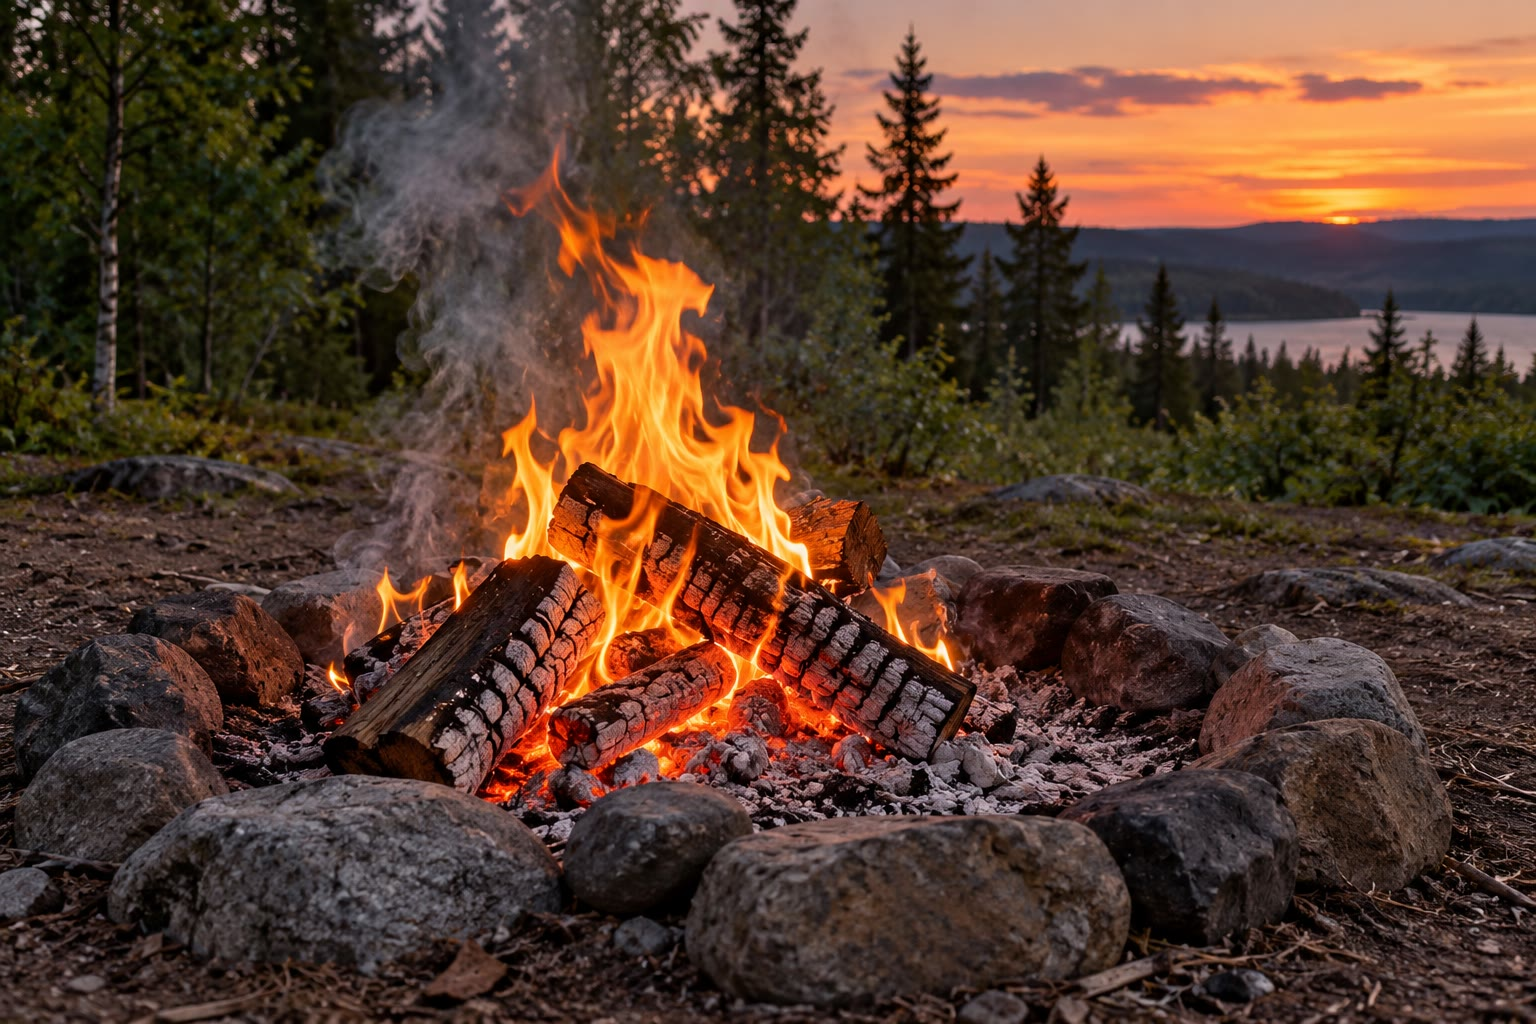
\includegraphics[width=0.6\linewidth]{images/book1/ai/g4-campfire.jpg}

{\small Una hoguera: madera, \omterm{def:g4:air-a-mixture-of-gases:air}{aire} y una cerilla --- y después, ceniza y
humo.}
\end{omfigure}

\section{Los combustibles}

\begin{definition}[Combustible]\label{def:g4:what-a-fire-needs:fuel}
Un \emph{combustible}\index{combustible} es un material que puede \omterm{def:g4:what-a-fire-needs:burning}{arder}
y desprender calor y luz: la madera, el papel, el carbón, la cera de
una vela, el gas de una cocina, la gasolina, el gasóleo de calefacción.
\end{definition}

\begin{example}[Combustibles sólidos, líquidos y gaseosos]\label{ex:g4:what-a-fire-needs:fuels}
La madera, el papel, el carbón y la cera de una vela son \omterm{def:g4:what-a-fire-needs:fuel}{combustibles}
sólidos. La gasolina y el gasóleo de calefacción son \omterm{def:g4:what-a-fire-needs:fuel}{combustibles}
líquidos. El gas de la cocina y el gas de un mechero son \omterm{def:g4:what-a-fire-needs:fuel}{combustibles}
gaseosos.
\end{example}

\begin{remark}[No todo arde]\label{rem:g4:what-a-fire-needs:not}
La piedra, la arena, el vidrio y el agua no \omterm{def:g4:what-a-fire-needs:burning}{arden}: no son \omterm{def:g4:what-a-fire-needs:fuel}{combustibles}.
Por eso una chimenea se construye de piedra o de ladrillo, y por eso se
usan la arena y el agua para apagar fuegos.
\end{remark}

\section{El triángulo del fuego}

\begin{definition}[Triángulo del fuego]\label{def:g4:what-a-fire-needs:fire-triangle}
Un fuego necesita tres cosas a la vez: un \omterm{def:g4:what-a-fire-needs:fuel}{combustible}, el oxígeno del
\omterm{def:g4:air-a-mixture-of-gases:air}{aire} y calor para empezar. Estas tres cosas se dibujan como los tres
lados de un triángulo, el \emph{triángulo del fuego}\index{triangulo del fuego@triángulo del fuego}.
Si falta un lado, no hay fuego.
\end{definition}

\begin{omfigure}
\begin{tikzpicture}[font=\small]
  \coordinate (A) at (0,0); \coordinate (B) at (5,0); \coordinate (C) at (2.5,4.1);
  \draw[line width=3pt, brown!70!black] (A) -- (B);
  \draw[line width=3pt, omDef] (B) -- (C);
  \draw[line width=3pt, red!75!black] (C) -- (A);
  \node[below=4pt, font=\small\bfseries, brown!60!black] at (2.5,0) {combustible};
  \node[right=4pt, font=\small\bfseries, omDef] at (3.75,2.05) {oxígeno (del aire)};
  \node[left=4pt, font=\small\bfseries, red!75!black] at (1.25,2.05) {calor (para empezar)};
  % a flame in the middle
  \fill[orange!80] (2.5,0.55) .. controls (1.95,1.15) and (2.35,1.75) .. (2.55,2.3)
    .. controls (2.75,1.75) and (3.05,1.15) .. (2.5,0.55);
  \fill[yellow!80] (2.5,0.7) .. controls (2.25,1.05) and (2.4,1.35) .. (2.52,1.65)
    .. controls (2.62,1.35) and (2.75,1.05) .. (2.5,0.7);
\end{tikzpicture}

{\small El \omterm{def:g4:what-a-fire-needs:fire-triangle}{triángulo del fuego}: \omterm{def:g4:what-a-fire-needs:fuel}{combustible}, oxígeno y calor, los tres
juntos.}
\end{omfigure}

\begin{example}[Encender una cerilla]\label{ex:g4:what-a-fire-needs:match}
Se frota la cabeza de una cerilla contra el lateral de su caja. El
frotamiento la calienta lo bastante para que empiece a \omterm{def:g4:what-a-fire-needs:burning}{arder}: es el
lado del calor del triángulo. La madera de la cerilla es el \omterm{def:g4:what-a-fire-needs:fuel}{combustible},
y el \omterm{def:g4:air-a-mixture-of-gases:air}{aire} aporta el oxígeno.
\end{example}

\begin{example}[Soplar sobre las brasas]\label{ex:g4:what-a-fire-needs:embers}
Unas brasas incandescentes que parecen casi apagadas vuelven a echar
llamas cuando alguien sopla sobre ellas: al soplar llega más \omterm{def:g4:air-a-mixture-of-gases:air}{aire}, y por
tanto más oxígeno, al \omterm{def:g4:what-a-fire-needs:fuel}{combustible} que todavía está caliente.
\end{example}

\section{Al arder se forman sustancias nuevas}

\begin{definition}[Arder; combustión]\label{def:g4:what-a-fire-needs:burning}
Un \omterm{def:g4:what-a-fire-needs:fuel}{combustible} \emph{arde}\index{arder} cuando toma oxígeno del \omterm{def:g4:air-a-mixture-of-gases:air}{aire} y
desprende calor y luz. Los químicos llaman a esto una
\emph{combustión}\index{combustion@combustión}. Durante una combustión se gastan el
\omterm{def:g4:what-a-fire-needs:fuel}{combustible} y el oxígeno, y aparecen sustancias nuevas: humo, ceniza,
dióxido de carbono y vapor de agua.
\end{definition}

\begin{proposition}[Una combustión no tiene vuelta atrás]\label{prop:g4:what-a-fire-needs:new}
La ceniza y el humo de un fuego no vuelven a convertirse en madera, por
mucho que esperemos. Al \omterm{def:g4:what-a-fire-needs:burning}{arder} se forman sustancias nuevas que antes no
estaban; el \omterm{def:g4:what-a-fire-needs:fuel}{combustible} ha desaparecido para siempre.
\end{proposition}

\begin{inthelab}[Un vaso frío sobre una vela]
El profesor sostiene un momento, boca abajo, un vaso de precipitados de
vidrio frío y seco encima de la llama de una vela. El interior del vaso
se empaña con gotitas de agua: el vapor de agua que produce la vela al
\omterm{def:g4:what-a-fire-needs:burning}{arder} ha vuelto a hacerse líquido sobre el vidrio frío. Una vela que
\omterm{def:g4:what-a-fire-needs:burning}{arde} produce agua, y también dióxido de carbono, que se puede detectar
con una prueba que veremos en un capítulo posterior.
\end{inthelab}

\begin{omfigure}
\begin{tikzpicture}[font=\small, scale=1.3]
  % candle
  \fill[white, draw=black!50] (-0.25,0) rectangle (0.25,1.2);
  \draw[black!70] (0,1.2) -- (0,1.33);
  \fill[orange!85] (0,1.3) .. controls (-0.16,1.5) and (-0.06,1.75) .. (0,1.95)
    .. controls (0.06,1.75) and (0.16,1.5) .. (0,1.3);
  \fill[yellow!85] (0,1.36) .. controls (-0.08,1.5) and (-0.03,1.62) .. (0,1.72)
    .. controls (0.03,1.62) and (0.08,1.5) .. (0,1.36);
  % upturned cold beaker above
  \pic[transform shape, rotate=180] at (0,4.3) {beaker={0}{white}};
  \foreach \x/\y in {-0.6/3.9,-0.45/4.1,-0.2/3.95,0.1/4.15,0.35/3.9,0.6/4.05,
                     -0.7/3.5,0.7/3.4,-0.72/3.0,0.72/2.9}
    \fill[omDef!55] (\x,\y) circle (0.035);
  \draw[<-, omProp, thick] (0.68,3.95) -- (2.0,4.2) node[right, text=black]
    {gotitas de agua};
  \draw[<-, omProp, thick] (0.85,3.2) -- (2.0,3.3) node[right, text=black]
    {vaso frío, boca abajo};
  \draw[<-, omProp, thick] (0.15,1.7) -- (2.0,1.9) node[right, text=black]
    {la llama: cera que arde};
  \draw[<-, omProp, thick] (0.3,0.6) -- (2.0,0.7) node[right, text=black]
    {cera de la vela: el combustible};
\end{tikzpicture}

{\small Un vaso frío sostenido encima de una vela se empaña: la cera que
\omterm{def:g4:what-a-fire-needs:burning}{arde} produce vapor de agua.}
\end{omfigure}

\begin{example}[En qué se convierte un tronco]\label{ex:g4:what-a-fire-needs:log}
Un tronco de unos pocos kilos se reduce, al \omterm{def:g4:what-a-fire-needs:burning}{arder}, a un montoncito de
ceniza. La mayor parte de la madera no se ha esfumado: junto con el
oxígeno del \omterm{def:g4:air-a-mixture-of-gases:air}{aire}, se ha convertido en humo, dióxido de carbono y vapor
de agua, que son gases y se alejan hacia el cielo.
\end{example}

\section{Apagar un fuego}

\begin{method}[Apagar un fuego: quitar un lado]\label{met:g4:what-a-fire-needs:out}
Para apagar un fuego, se quita un lado del \omterm{def:g4:what-a-fire-needs:fire-triangle}{triángulo del fuego}:
\begin{itemize}
  \item \textbf{quitar el oxígeno}: cubrir el fuego con una manta
        ignífuga, una tapa o arena, para que el \omterm{def:g4:air-a-mixture-of-gases:air}{aire} no llegue a él;
  \item \textbf{quitar el calor}: echar agua sobre la madera o el papel
        que \omterm{def:g4:what-a-fire-needs:burning}{arden}, lo que los enfría por debajo del punto en que pueden
        \omterm{def:g4:what-a-fire-needs:burning}{arder};
  \item \textbf{quitar el \omterm{def:g4:what-a-fire-needs:fuel}{combustible}}: cerrar la llave del gas, o
        desbrozar las plantas secas alrededor de un incendio forestal.
\end{itemize}
\end{method}

\begin{omfigure}
\begin{tikzpicture}[font=\small, scale=0.7]
  \foreach \k/\lab/\side in {0/{una manta: sin oxígeno}/1, 1/{agua: sin calor}/2,
                              2/{gas cerrado: sin combustible}/0} {
    \begin{scope}[xshift=\k*6.2cm]
      \coordinate (A) at (0,0); \coordinate (B) at (4,0); \coordinate (C) at (2,3.3);
      \pgfmathsetmacro\oa{\side==0 ? 0.2 : 1}
      \pgfmathsetmacro\ob{\side==1 ? 0.2 : 1}
      \pgfmathsetmacro\oc{\side==2 ? 0.2 : 1}
      \draw[line width=2.5pt, brown!70!black, opacity=\oa] (A) -- (B);
      \draw[line width=2.5pt, omDef, opacity=\ob] (B) -- (C);
      \draw[line width=2.5pt, red!75!black, opacity=\oc] (C) -- (A);
      \ifnum\side=0 \draw[line width=1.4pt, black] (1.6,-0.4) -- (2.4,0.4) (1.6,0.4) -- (2.4,-0.4);\fi
      \ifnum\side=1 \draw[line width=1.4pt, black] (2.6,1.25) -- (3.4,2.05) (2.6,2.05) -- (3.4,1.25);\fi
      \ifnum\side=2 \draw[line width=1.4pt, black] (0.6,1.25) -- (1.4,2.05) (0.6,2.05) -- (1.4,1.25);\fi
      \node[align=center, anchor=north] at (2,-0.6) {\lab};
    \end{scope}
  }
\end{tikzpicture}

{\small Tres maneras de apagar un fuego, cada una quitando un lado del
triángulo (tachado): el oxígeno, el calor o el \omterm{def:g4:what-a-fire-needs:fuel}{combustible}.}
\end{omfigure}

\begin{omfigure}
\begin{minipage}[t]{0.48\linewidth}\centering
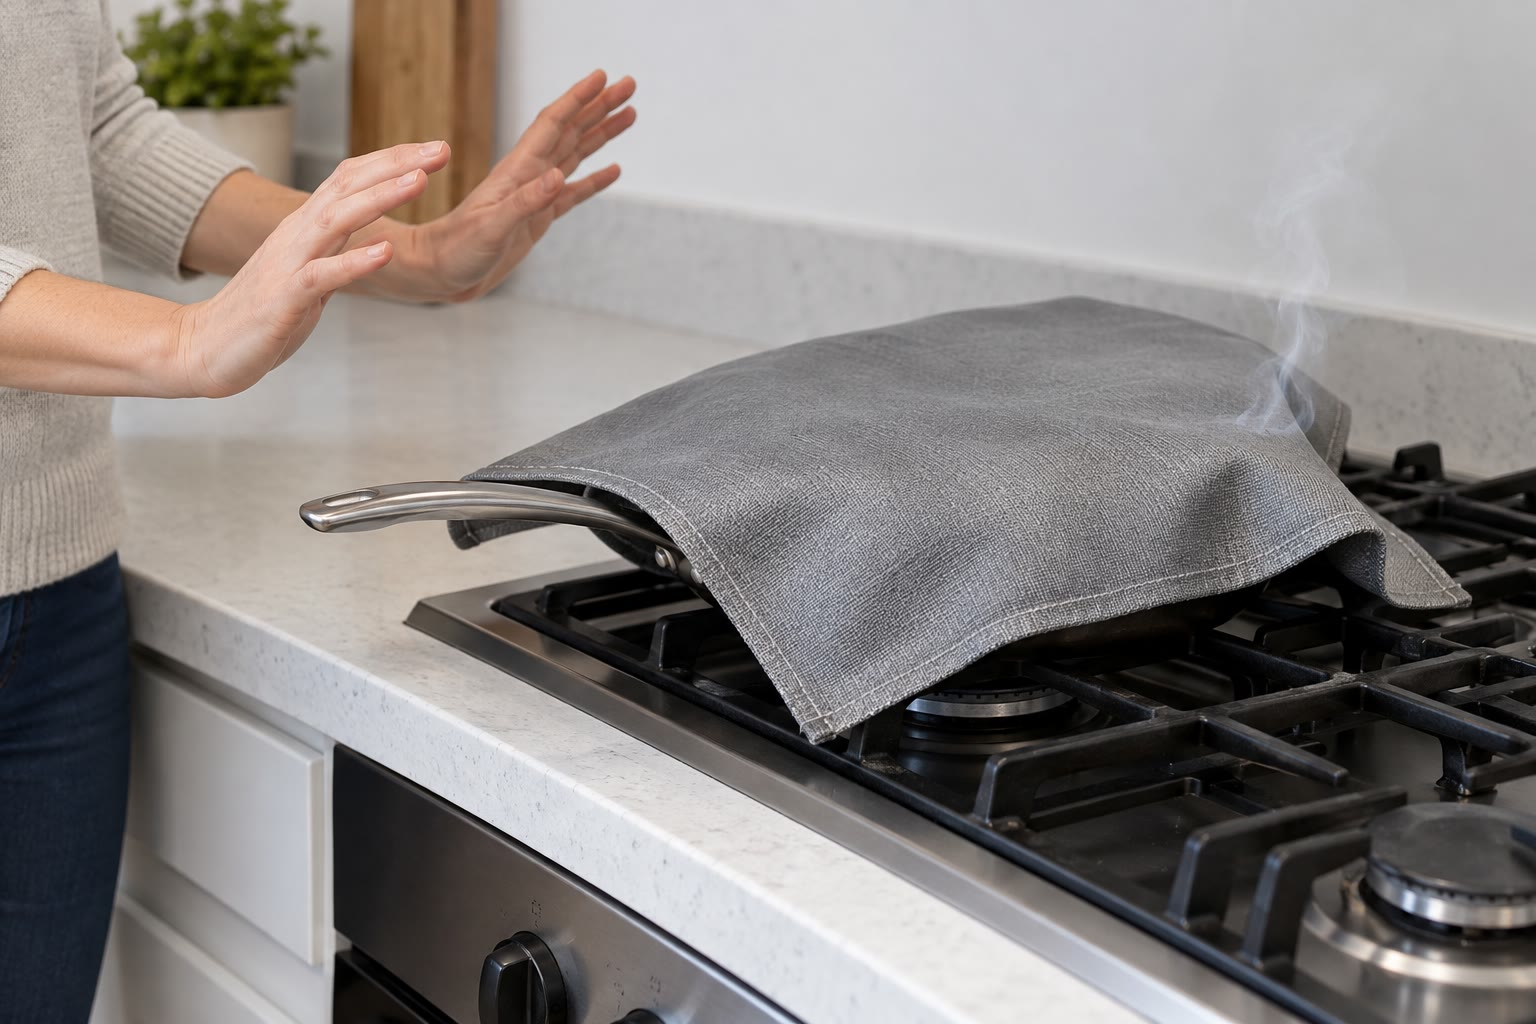
\includegraphics[width=\linewidth,height=4.6cm,keepaspectratio]{images/book1/ai/g4-fire-blanket.jpg}

{\small Una manta ignífuga sobre una sartén: el \omterm{def:g4:air-a-mixture-of-gases:air}{aire} ya no puede llegar
al fuego.}
\end{minipage}\hfill
\begin{minipage}[t]{0.48\linewidth}\centering
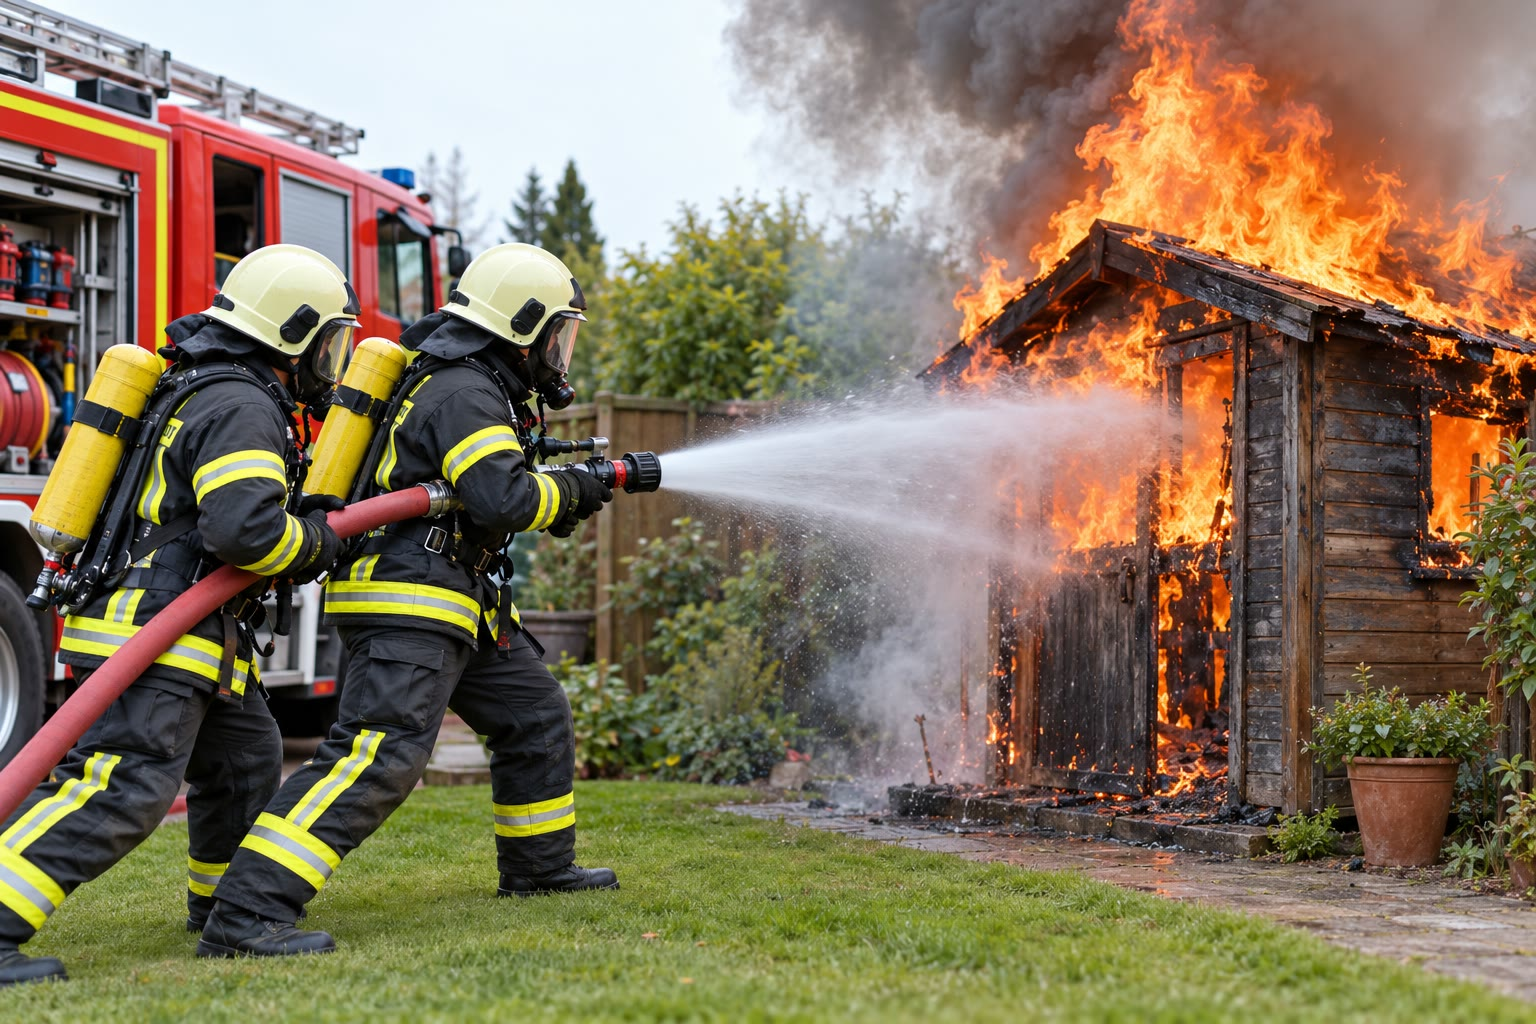
\includegraphics[width=\linewidth,height=4.6cm,keepaspectratio]{images/book1/ai/g4-firefighters.jpg}

{\small Unos bomberos lanzan agua para enfriar un cobertizo en llamas.}
\end{minipage}
\end{omfigure}

\section{Seguridad ante el fuego}

\begin{remark}[Nunca agua sobre una sartén con aceite ardiendo]\label{rem:g4:what-a-fire-needs:oil}
Si el aceite de una sartén se prende fuego, nadie debe echarle agua: el
agua hierve de golpe bajo el aceite y lanza aceite \omterm{def:g4:what-a-fire-needs:burning}{ardiendo} fuera de la
sartén. Un adulto apaga el gas o la placa y cubre la sartén con una tapa
o con una manta ignífuga.
\end{remark}

\begin{safety}{\ghs{GHS02}\ghs{GHS04}}
% ledger: ghs:butane
El gas de un mechero o de un cartucho de camping es butano. Su
pictograma de la llama (GHS02) significa: extremadamente inflamable,
mantener lejos de llamas y chispas. El pictograma de la bombona de gas
(GHS04) significa: gas guardado a presión.
\end{safety}

\begin{proposition}[Qué hacer si hay un incendio]\label{prop:g4:what-a-fire-needs:safety}
El humo es el primer peligro de un incendio: está caliente, oculta la
salida y es venenoso respirarlo. Un detector de humo en el techo pita
con fuerza en cuanto el humo llega a él. Si hay un incendio: sal,
agáchate por debajo del humo, cierra las puertas al pasar y llama a los
bomberos desde fuera. No vuelvas a entrar nunca.
\end{proposition}

\begin{omfigure}
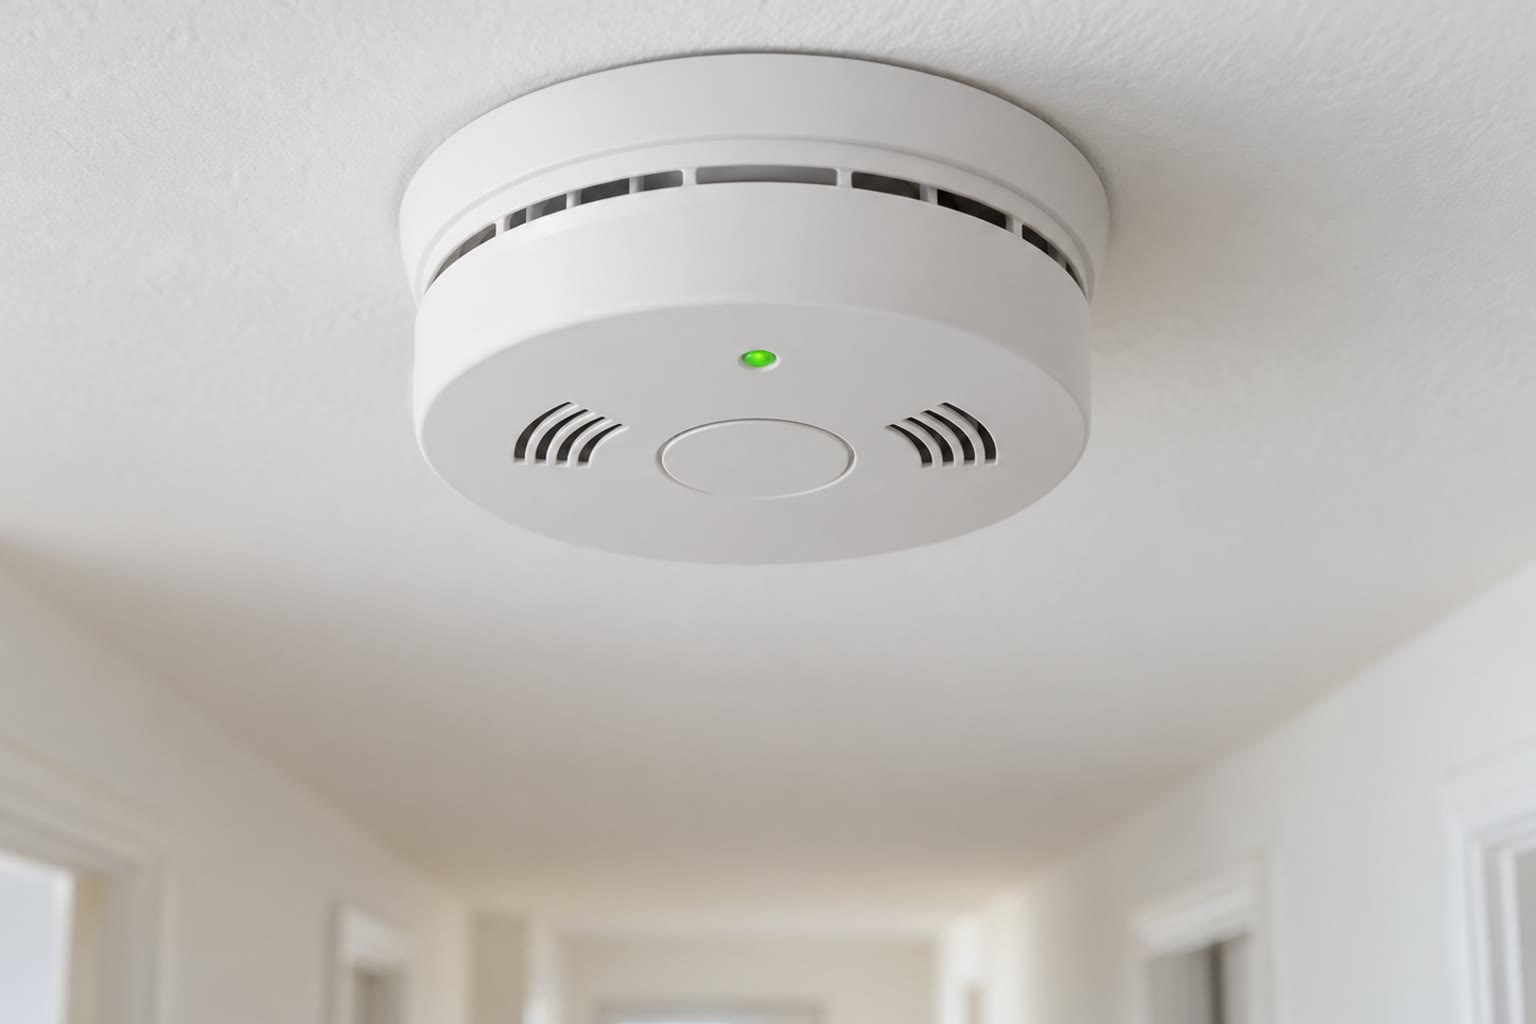
\includegraphics[width=0.42\linewidth]{images/book1/ai/g4-smoke-alarm.jpg}

{\small Un detector de humo: suena en cuanto el humo llega a él.}
\end{omfigure}

\section{Ejercicios}

\begin{exercise}[$\star$]\label{exo:g4:what-a-fire-needs:1}
Nombra los tres lados del \omterm{def:g4:what-a-fire-needs:fire-triangle}{triángulo del fuego}.
\end{exercise}

\begin{exercise}[$\star$]\label{exo:g4:what-a-fire-needs:2}
¿Cuáles de estos son \omterm{def:g4:what-a-fire-needs:fuel}{combustibles}: madera, arena, cera de vela, vidrio,
gasolina, agua, papel?
\end{exercise}

\begin{exercise}[$\star$]\label{exo:g4:what-a-fire-needs:3}
Se echa una manta ignífuga sobre un fuego pequeño. ¿Qué lado del
\omterm{def:g4:what-a-fire-needs:fire-triangle}{triángulo del fuego} quita?
\end{exercise}

\begin{exercise}[$\star$]\label{exo:g4:what-a-fire-needs:4}
Los bomberos lanzan agua sobre un cobertizo en llamas. ¿Qué lado del
\omterm{def:g4:what-a-fire-needs:fire-triangle}{triángulo del fuego} quita el agua?
\end{exercise}

\begin{exercise}[$\star$]\label{exo:g4:what-a-fire-needs:5}
Nombra tres sustancias nuevas que se forman cuando \omterm{def:g4:what-a-fire-needs:burning}{arde} la madera.
\end{exercise}

\begin{exercise}[$\star$]\label{exo:g4:what-a-fire-needs:6}
¿Por qué, al soplar sobre unas brasas incandescentes, vuelven a echar
llamas?
\end{exercise}

\begin{exercise}[$\star$]\label{exo:g4:what-a-fire-needs:7}
Un vaso frío sostenido encima de una vela se empaña. ¿Qué sustancia
nueva ha producido la vela?
\end{exercise}

\begin{exercise}[$\star$]\label{exo:g4:what-a-fire-needs:8}
¿Qué es lo primero que debes hacer si suena un detector de humo y ves
humo?
\end{exercise}

\begin{exercise}[$\star$]\label{exo:g4:what-a-fire-needs:9}
Mira la figura de los tres triángulos pequeños. ¿Qué lado está tachado
cuando se cierra el gas?
\end{exercise}

\begin{exercise}[$\star\star$]\label{exo:g4:what-a-fire-needs:10}
Para detener un incendio forestal, los bomberos cortan a veces una
franja ancha de árboles delante del fuego. ¿Qué lado del \omterm{def:g4:what-a-fire-needs:fire-triangle}{triángulo del
fuego} están quitando?
\end{exercise}

\begin{exercise}[$\star\star$]\label{exo:g4:what-a-fire-needs:11}
Un tronco pesa mucho más que su ceniza. ¿Ha desaparecido una parte del
tronco? Explica adónde ha ido.
\end{exercise}
